% Chapter Template

\chapter{Ensayos y resultados} % Main chapter title

\label{Chapter4} % Change X to a consecutive number; for referencing this chapter elsewhere, use \ref{ChapterX}

%----------------------------------------------------------------------------------------
%	CHAPTER 4
%----------------------------------------------------------------------------------------

En este capítulo se explica cómo se llevaron a cabo las pruebas de validación de hardware y software a las que fue sometido el dispositivo, los bancos de ensayos, instrumentos utilizados y los resultados obtenidos.

\section{Instrumental utilizado}

Para poder ejecutar las pruebas de integración de hardware y software se requirió del uso de una variedad de instrumentos y componentes en los bancos de ensayos. La tabla \ref{tab:instrumentos} lista los detalles de cada uno de ellos.

\begin{table}[H]
	\centering
	\caption{Lista de instrumental utilizado.}
	\begin{tabular}{p{3cm} c p{6cm}}
		\toprule
		\textbf{Item} & \textbf{Modelo} & \textbf{Descripción} \\
		\midrule
		Multímetro			& UNI-T UT61A		& Multímetro digital autorango de alta precisión. \\
		Fuente de tensión	& KM GP-300ATX		& Fuente de computadora de 400 W. \\
		Resistencia de potencia variable		& AVT05006E25R00KE	& Resistencia de potencia de alambre bobinado de 25 Ohm / 50 W. \\
		Potenciómetro							& 3590S-1-201L & Potenciómetro de 200 Ohm / 2 W y 10 vueltas para panel. \\
		Conversor USB a UART					& EM7-6043		& Conversor USB a serie TTL CH-340. \\
		Cables varios							& - 			& Cables dupont y unipolar de 2,5 mm2. \\
		PC										& -				& Computadora de escritorio con software PuTTY (cliente de terminal). \\
		\bottomrule
		\hline
	\end{tabular}
	\label{tab:instrumentos}
\end{table}

\section{Banco de ensayos}

En la figura \ref{fig:setupEnsayos} se puede ver una foto del banco de ensayos completo con todos los instrumentos y hardware utilizado.

%\begin{figure}[H]
%\centering
%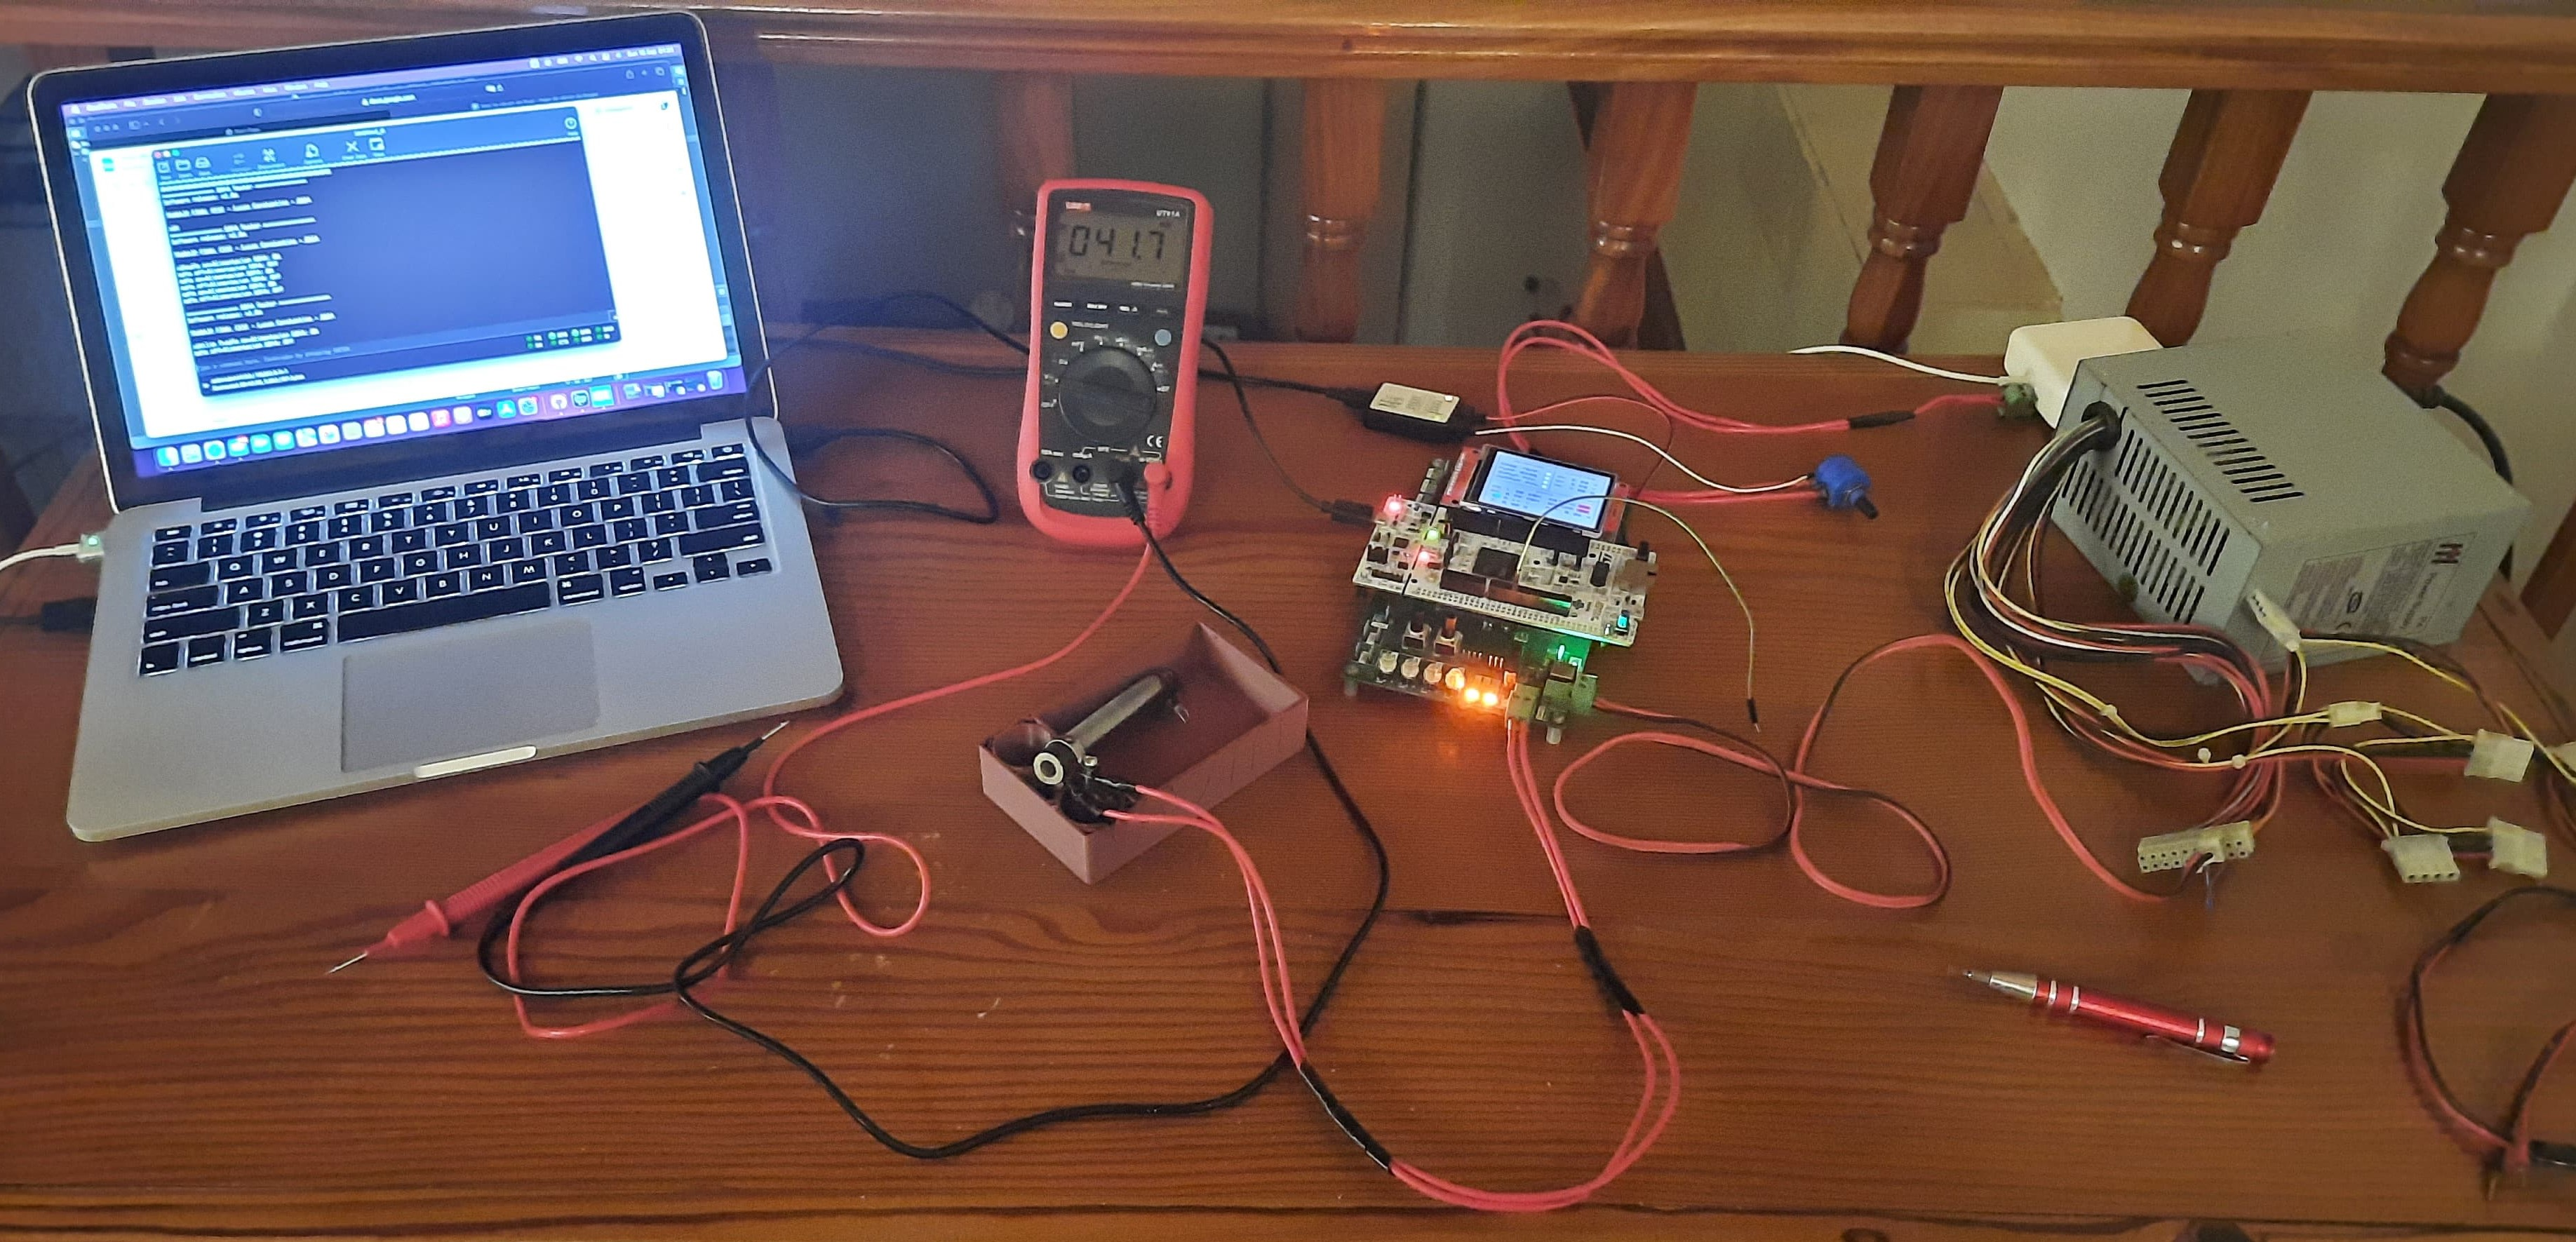
\includegraphics[width=0.75\textwidth]{./Figures/setupEnsayos.png}
%\caption{Banco de ensayos}
%\label{fig:setupEnsayos}
%\end{figure}

\section{Pruebas de hardware}
\label{sec:pruebasHW}

El diseño del hardware de la placa ensamblada no es de gran complejidad y el funcionamiento de sus distintas partes resulta trivial. En general, solo basta con medir continuidad o valores de tensión en ciertos puntos para concluir que funcionan correctamente. Por esta razón, se omite especificar las pruebas, a excepción de las del monitor de corriente, ya que es el único caso en el que es necesario realizar mediciones.

\subsection{Pruebas del monitor de corriente}

En el circuito del monitor de corriente lo que se desea verificar es que a la salida del amplificador se obtenga una tensión proporcional al valor de corriente que circula. La constante de conversión surge de multiplicar el valor de la resistencia de sensado (10 mOhm) por la constante de amplificación del circuito integrado (100 V/V), lo que resulta en un valor de 1 V/A. Por lo tanto, la conversión entre corriente y tensión es unitaria.

Para realizar las mediciones se conecta la entrada de tensión a 5 V, un reóstato en la salida de tensión y se varía su valor de forma de recorrer desde 0 A hasta aproximadamente 4 A.

En la figura \ref{fig:testMonCorr1} se puede ver el valor de tensión medido (en azul) junto con el valor teórico (recta en verde) en función de la corriente que circula por la carga. 

%\begin{figure}[H]
%\centering
%\includegraphics[width=0.9\textwidth]{./Figures/testMonCorr1.png}
%\caption{Valor de tensión de salida del monitor de corriente.}
%\label{fig:testMonCorr1}
%\end{figure}

Esta diferencia entre el valor de la constante medida y el teórico se la puede atribuir principalmente a dos efectos: la dispersión del valor de la resistencia de sensado y el error de la ganancia del circuito integrado (el cual está especificado en un 0,2\% como máximo).

\section{Pruebas de firmware}
\label{sec:pruebasFW}



\subsection{Pruebas del monitor de tensión}

Para realizar las mediciones se conecta la entrada de tensión a una fuente variable y se lee directamente el valor medido que muestra la pantalla LCD. Se toman varios valores en el rango entre 0 V y 5 V.

En la figura \ref{fig:testMonTens} se puede ver la comparación entre el valor de tensión de alimentación medido con el multímetro (azul) y el valor mostrado en la pantalla LCD (verde).

%\begin{figure}[H]
%\centering
%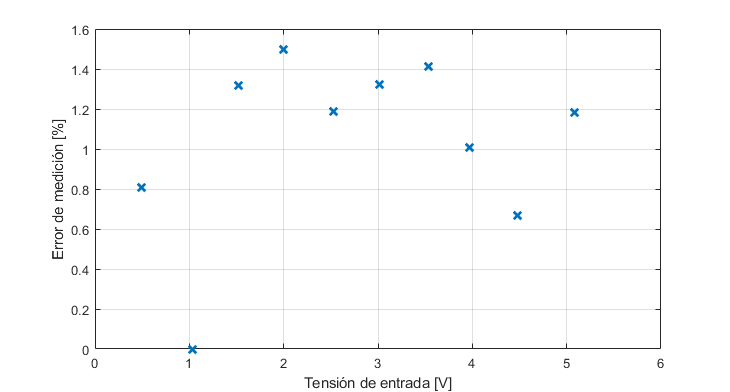
\includegraphics[width=0.9\textwidth]{./Figures/testMonTens.png}
%\caption{Detección de alarma y apagado de salida del EDFA.}
%\label{fig:testMonTens}
%\end{figure}

\subsection{Pruebas del monitor de corriente}

En la figura \ref{fig:detecAlarm} se puede ver la comparación entre el valor de corriente de alimentación medido con el tester (azul) y el valor mostrado en la pantalla LCD (verde).

%\begin{figure}[H]
%\centering
%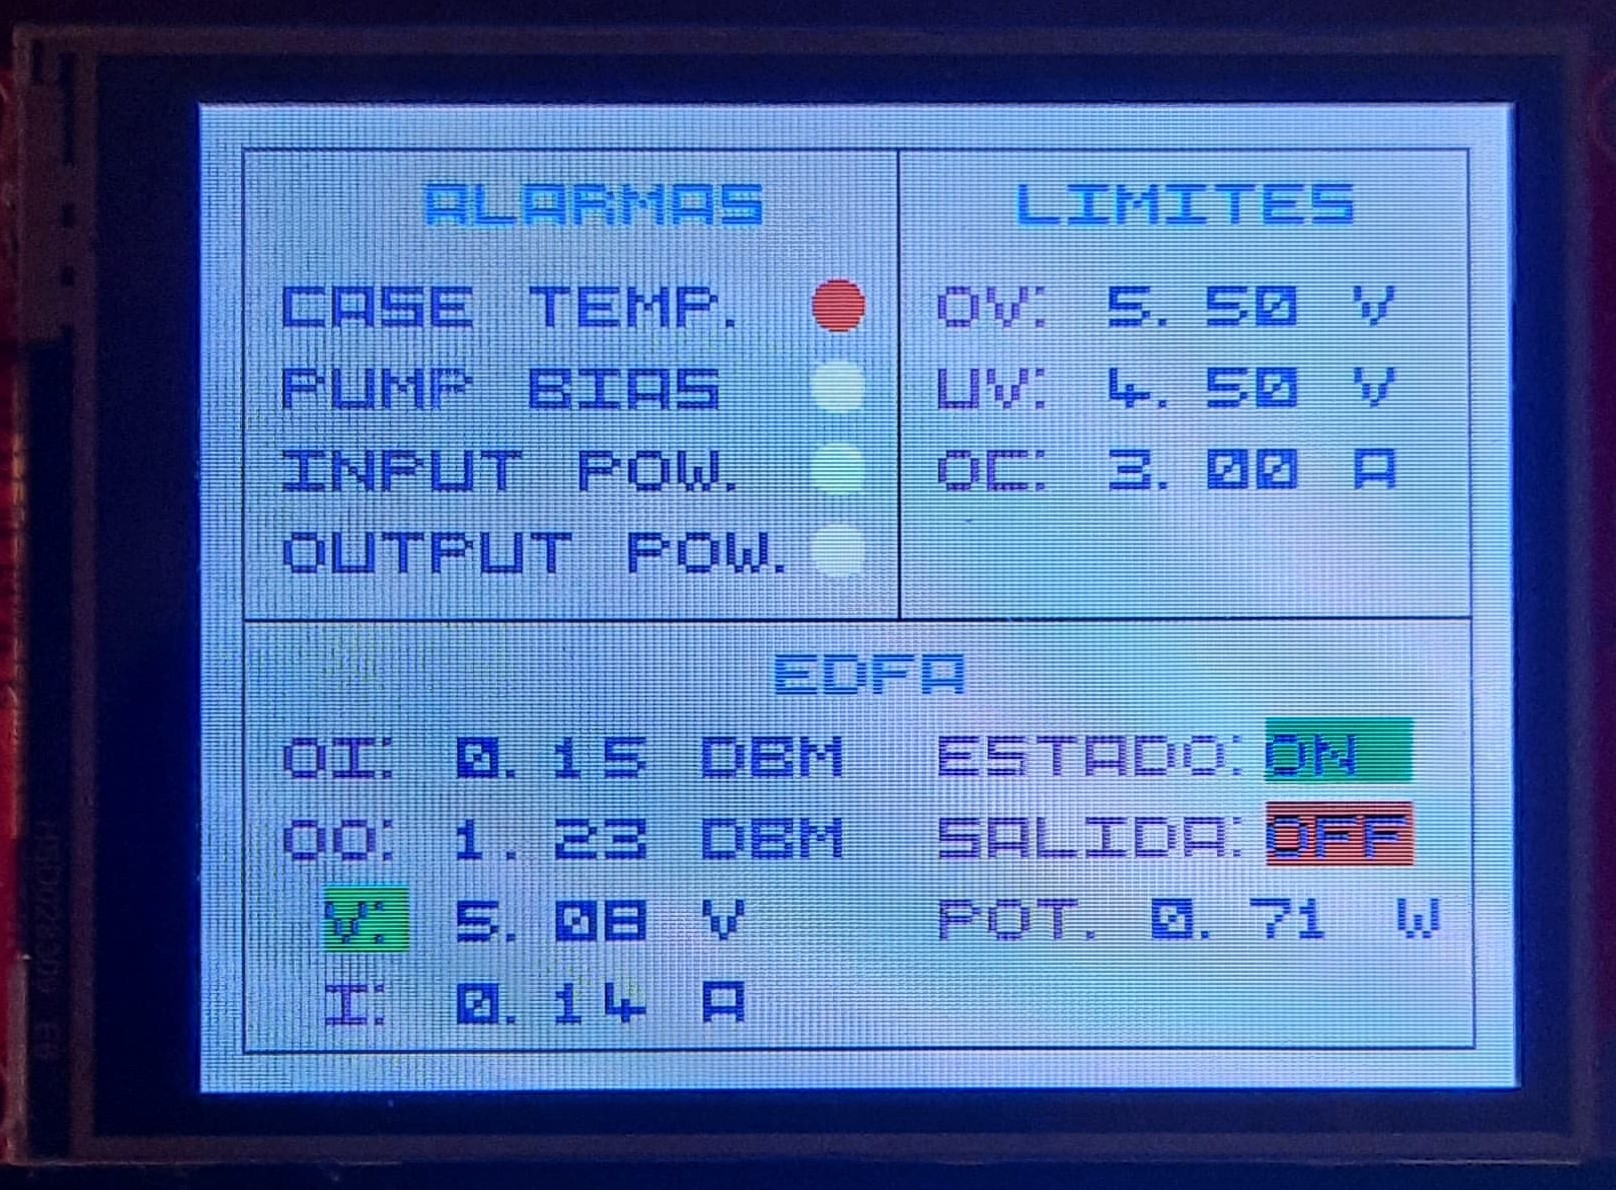
\includegraphics[width=0.9\textwidth]{./Figures/detecAlarm.png}
%\caption{Detección de alarma y apagado de salida del EDFA.}
%\label{fig:detecAlarm}
%\end{figure}

Observando el gráfico se desprende que la medición tiene cierta dispersión, siendo máxima al rededor de los X A. Tomando todos los valores en el rango medido resulta un error promedio aproximado del X \% respecto del valor real.

\subsection{Pruebas de la pantalla LCD}



\subsection{Pruebas de la pantalla táctil}



\subsection{Pruebas de la comunicación UART}



\section{Pruebas de integración}
\label{sec:pruebasInt}

Las pruebas de integración tienen como objetivo verificar el cumplimiento de los requerimientos establecidos en el documento \ref{DOC_REQ} y mencionados en la sección \ref{sec:reqs}. Al hacer esto se valida la correcta interacción entre el hardware y el firmware, es decir, el funcionamiento del sistema como una unidad.

\subsection{Funcionamiento normal}

En la figura \ref{fig:funcNorm} se puede ver una imagen de la pantalla LCD durante el funcionamiento normal, con el amplificador alimentado y su salida óptica prendida.


%\begin{figure}[H]
%\centering
%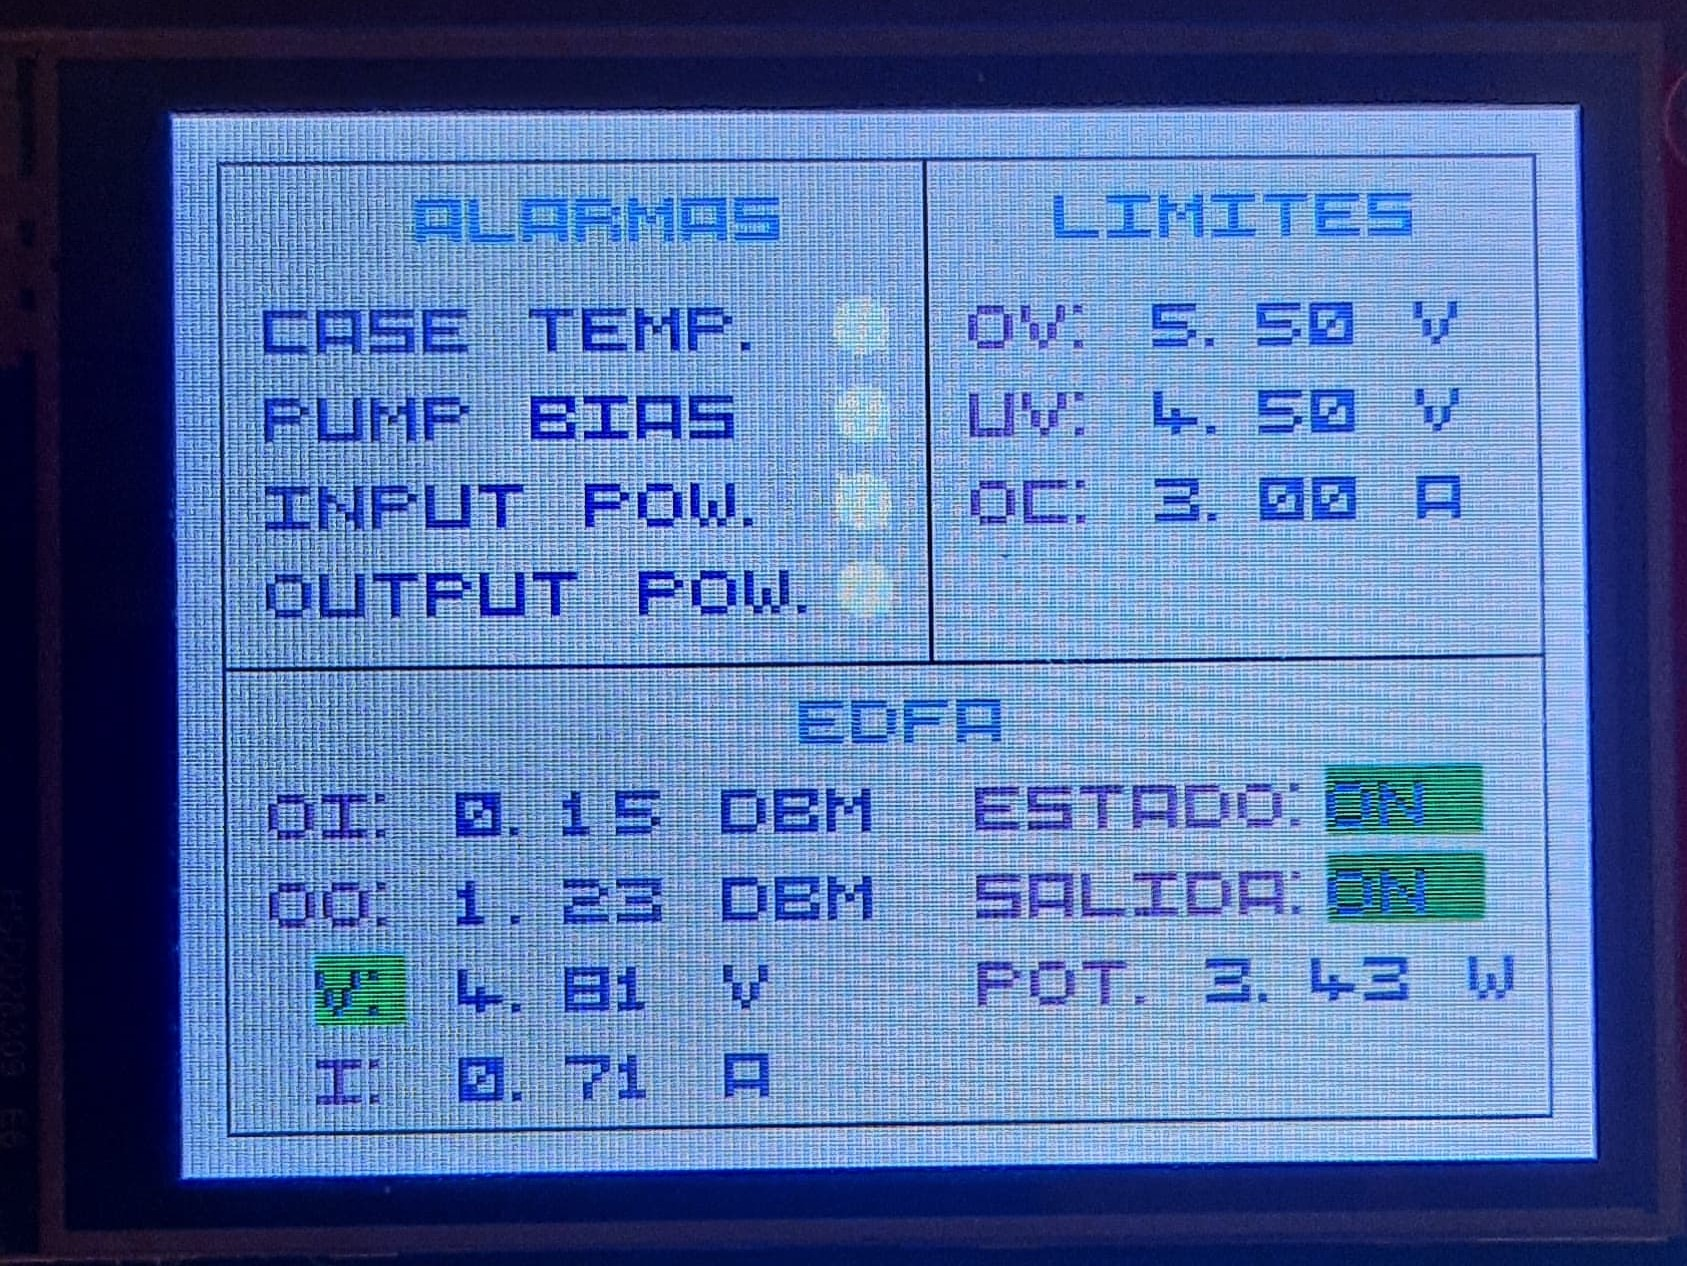
\includegraphics[width=0.9\textwidth]{./Figures/funcNorm.png}
%\caption{Detección de alarma y apagado de salida del EDFA.}
%\label{fig:funcNorm}
%\end{figure}

\subsection{Apagado de salida del EDFA}

En la figura \ref{fig:detecAlarm} se puede ver la conmutación de la señal de control OUT MUTE cuando la señal de alarma X se activa. 

%\begin{figure}[H]
%\centering
%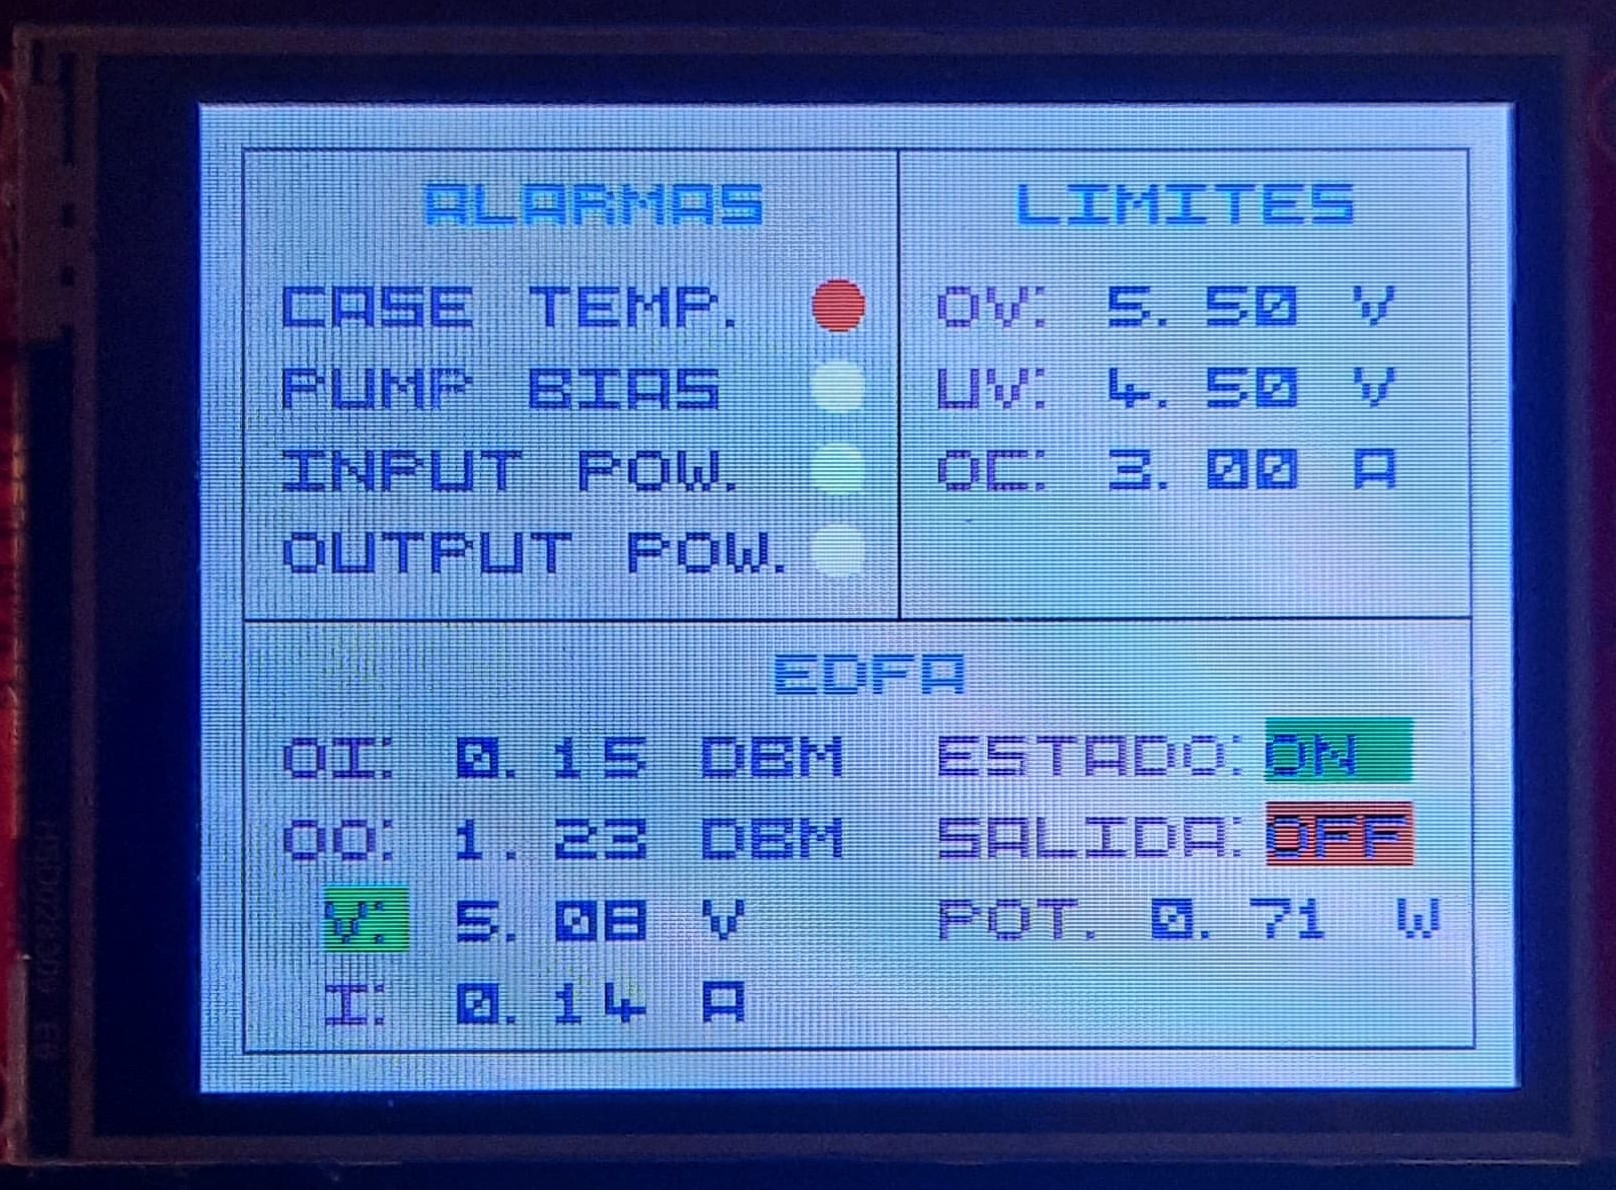
\includegraphics[width=0.9\textwidth]{./Figures/detecAlarm.png}
%\caption{Detección de alarma y apagado de salida del EDFA.}
%\label{fig:detecAlarm}
%\end{figure}

En la figura anterior se puede observar que el tiempo de retardo que existe entre la detección de la alarma del EDFA y el apagado de la salida óptica es de aproximadamente X ms, lo cual cumple con el requerimiento X especificado en la sección \ref{sec:reqs}.

\subsection{Desconexión de alimentación del EDFA}

En la figura \ref{fig:detecOC} se puede ver la conmutación de la señal que controla la activación del relé cuando la señal de alarma de sobrecorriente se activa. 

%\begin{figure}[H]
%\centering
%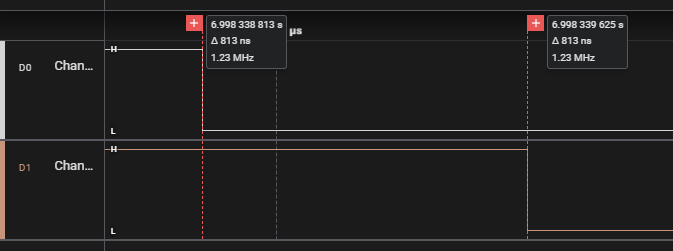
\includegraphics[width=0.9\textwidth]{./Figures/detecOC.png}
%\caption{Detección de sobrecorriente y desconexión del EDFA.}
%\label{fig:detecOC}
%\end{figure}

En la figura anterior se puede observar que el tiempo de retardo que existe entre la detección de la sobrecorriente y la desconexión del relé es de aproximadamente X ms, lo cual cumple con el requerimiento X especificado en la sección \ref{sec:reqs}.